\documentclass[12pt]{ociamthesis}  % default square logo 
%\documentclass[12pt,beltcrest]{ociamthesis} % use old belt crest logo
%\documentclass[12pt,shieldcrest]{ociamthesis} % use older shield crest logo

%load any additional packages
\usepackage{hyperref}
\usepackage{amssymb}
\usepackage{amsmath}
\usepackage{longtable}
%\usepackage{listings} %code listing, memasukkan code

%input macros (i.e. write your own macros file called mymacros.tex 
%and uncomment the next line)
%\include{mymacros}

\title{Panduan Penanganan\\[1ex]     %your thesis title,
        \textit{Error} Aplikasi}   %note \\[1ex] is a line break in the title

\author{Rolly Maulana Awangga\\Github : github.com/awangga\\
M. Innal Kariem\\Github : github.com/karieminnal \\
Rayhan Prastya\\Github : github.com/rayprastya\\
}             %your name
\college{}  %your college

%\renewcommand{\submittedtext}{change the default text here if needed}
\degree{Applied Bachelor Program of Informatics Engineering}     %the degree
\degreedate{Bandung\\ 2019}         %the degree date

%end the preamble and start the document
\begin{document}

%this baselineskip gives sufficient line spacing for an examiner to easily
%markup the thesis with comments
\baselineskip=18pt plus1pt

%set the number of sectioning levels that get number and appear in the contents
\setcounter{secnumdepth}{3}
\setcounter{tocdepth}{3}


\maketitle                  % create a title page from the preamble info
\begin{dedication}
`Jika Kamu tidak dapat menahan lelahnya belajar, \\
Maka kamu harus sanggup menahan perihnya Kebodohan.'\\ 
~Imam Syafi'i~\\
\end{dedication}        % include a dedication.tex file
\begin{acknowledgements}
Puji dan syukur kami panjatkan hadirat Allah S.W.T atas rahmat dan karunia-Nya kami dapat menyelesaikan panduan penanganan \textit{error} aplikasi ini.
Dan tidak lupa juga kami ucapkan kepada rekan dan para dosen yang namanya tidak dapat kami sebutkan satu per satu, yang telah membantu kami dalam proses pengerjaan panduan penanganan \textit{error} aplikasi ini, diharapkan panduan ini dapat berguna bagi para pembaca dan juga menjadi acuan baik itu dalam pemahaman tentang berbagai macam jenis \textit{error} atau proses penyelesaian suatu \textit{error}.
\end{acknowledgements}   % include an acknowledgements.tex file
\begin{abstract}
	Panduan Penanganan \textit{Error} Aplikasi ini dibuat dengan tujuan memberikan pemahaman mendalam tentang \textit{error} kepada para sivitas akademika.
	Dimulai dari pengenalan berbagai macam \textit{error} hingga cara penyelesaiannya, Panduan ini akan menjabarkan tentang pengenalan berbagai macam \textit{error}, standar penulisan sebuah program, hingga cara penyelesaiannya. Dengan demikian diharapkan semua sivitas akademika dapat memahami berbagai jenis \textit{error} yang terdapat pada suatu program, dan dapat mengatasi \textit{error} yang terdapat pada suatu program.
\end{abstract}          % include the abstract

\begin{romanpages}          % start roman page numbering
\tableofcontents            % generate and include a table of contents         
\end{romanpages}            % end roman page numbering

%now include the files of latex for each of the chapters etc
\chapter{Standar Perlengkapan}
\textit{Error} terjadi pada suatu program akibat ketidaksesuaian penyusunan suatu program dengan standar yang sudah ditetepkan.
Dalam kasus penangan \textit{error}, beberapa bahasa pemrograman memiliki \textit{IDE} yang merupakan singkatan dari \textit{Integrated Development Environment} yang dapat melakukan pengecekan \textit{error} secara \textit{realtime}. Disini kita membutuhkan \textit{IDE} dari suatu bahasa pemrograman yang memiliki \textit{variable explorer} . \textit{variable explorer} berfungsi menampilkan konten-konten apasaja yang ada di baris \textit{coding}-an kita, yang bertujuan untuk mempermudah kita untuk menyusun \textit{code} program. Jadi perlengkapan yang kita harus persiapkan adalah :

\begin{enumerate}
\item Bahasa pemorgraman
\item \textit{IDE} dari suatu bahasa pemrograman yang memiliki \textit{variable explorer}.
\end{enumerate}

\section{Jenis \textit{Error}}
\par 
\textit{Error} atau bisa disebut dengan kesalahan pada program memiliki berbagai jenis tipe, diantaranya :

\begin{enumerate}
\item 
\textit{Syntax errors}
\par 
\textit{Syntax errors} adalah \textit{error} yang diakibatkan oleh kesalahan dalam penulisan bahasa program yang tidak dapat dimengerti oleh \textit{compiler} , contohnya adalah sebagai berikut.

\begin{verbatim}
#include <stdio.h>

int main(void) {
    printf("Hello World!\n";
    return 0;
}
\end{verbatim}
 
Terdapat \textit{syntax error} pada program ini, \textit{syntax error} disini diakibatkan kurangnya tanda ")" pada akhir baris \textit{code} tersebut. Kurangnya "\;" , ")" , "]" , "\}" pada akhir atau awal baris \textit{code} juga dapat menyebabkan terjadinya \textit{syntax error}.

\item 
\textit{Semantic errors}
\par 
\textit{Semantic errors} terjadi akibat tidak tepatnya varibel dengan \textit{statement} yang sudah dibuat, ketidakjelasan logika pada program yang dibuat akan menimbulkan \textit{semantic error} contohnya adalah sebagai berikut.

\begin{verbatim}
public static void main(String[] args) {	
		String NPM;		
		NPM = "Rayhan";
		System.out.println(NPM);
	}
\end{verbatim}
\par 
Program ini akan menghasilkan \textit{semantic error},\textit{compiler} tetap dapat menjalan kan program tersebut,namun output yang dikeluarkan berupa String. jika output yang diinginkan berupa NPM yang bertipe data INT, maka tipe data yang diinputkan harus sesuai dengan output yang diinginkan.
\end{enumerate}
\chapter{Standar Penulisan Program}

\par 
Dalam pengerjaan suatu program, hendaknya baris \textit{code} yang kita buat sesuai standar dari penulisan program, karena setiap bahasa pemrograman memiliki aturan penulisannya sendiri-sendiri, contohnya pada bahasa C, bahasa C bersifat \textit{case sensitifity} dimana huruf kapital dan huruf kecil memiliki arti yang berbeda,contohnya pada gambar berikut.

\begin{verbatim}
#include <stdio.h>

int main(void) {
    printf("Hello World!\n");
    Return 0;
}
\end{verbatim}

\par 
Pada baris \textit{code} berikut terdapat parameter \textit{return} yang seharusnya diketik dengan huruf kecil, karena pada awalan \textit{parameter return} diketik menggunakan huruf kapital, sehingga baris \textit{code} tersebut menghasilkan \textit{error}.
\par 
Sehingga pada dasarnya, sebaiknya saat mengerjakan suatu program hendaknya mengikuti standar penulisan dari bahasa program tersebut dan terstruktur, agar memudahkan proses pengerjaan suatu program dan terlihat lebih rapi.

\section{Standar Penulisan Nama Variabel}
\par 
Setiap pemberian nama pada variabel hendaknya sesuai dengan isi/\textit{context} dari \textit{code} yang sedang dibuat, untuk mempermudah proses pengembangan sebuah program, contoh penamaan variabel yang baik adalah sebagai berikut.

\begin{verbatim}
	public static void main(String[] args) {	
		int NPM;		
		NPM = 1184069;
		System.out.println(NPM);
	}
\end{verbatim}

\par 
Didalam program tersebut terdapat sebuah variabel yang diberi nama NPM (Nomor Pokok Mahasiswa), variabel tersebut diberi nama NPM karena \textit{output} yang diharapkan nantinya adalah pencetakan Nomor Pokok Mahasiswa, jika variabel tersebut diberikan nama yang asal-asalan, hal ini akan mempersulit developer itu sendiri saat hendak menggunakan variabel itu kembali karena nama yang diberikan pada variabel itu asal-asalan.


\section{Standar Penamaan Fungsi}
\par 
Sama hal-nya dengan pemberian nama pada sebuah variabel, penamaan fungsi pada suatu program hendaknya disesuaikan dengan \textit{output}/isi dari proses fungsi tersebut, karena pemberian nama fungsi yang tidak sesuai dengan \textit{output} atau isi yang diharapkan hanya akan mempersulit developer dalam proses pengembangan sebuah aplikasi, contoh penamaan fungsi yang baik adalah sebagai berikut.

\begin{verbatim}
	def getURL(self,PROYEK):
		if PROYEK == '2':
			active_url = "https://cobahayo.herokuapp.com/"
		else:
			active_url = "https://proyek3d4tiv2.herokuapp.com/"
		return active_url
		
\end{verbatim}

\par 
Output dari program diatas ditunjukkan untuk mahasiswa yang hendak mengikuti proyek 2, yang nantinya jika mahasiswa menginput angka 2 ( Proyek 2 ), maka program akan mengaktifkan \textit{url} \url{"https://cobahayo.herokuapp.com/"} , jika fungsi tersebut diberikan nama yang asal-asalan, hal ini akan mempersulit developer dalam melakukan pengembangan pada aplikasi.

\section{Standar Pembuatan Fungsi}
\par 
Fungsi berfungsi untuk menjalankan suatu tugas yang ditulis dalam 1 blok \textit{code} yang akan dieksekusi apabila fungsi tersebut dipanggil pada program utama. Pembuatan suatu fungsi sebaiknya dibedakan sesuai dengan pekerjaan yang dilakukan oleh fungsi tersebut, tidak dianjurkan untuk mencampurkan berbagai macam pekerjaan pada 1 fungsi, hal ini dapat menimbulkan \textit{error}, sehingga sebaiknya fungsi dibuat untuk 1 pekerjaan saja. Tidak membuat 2 buah fungsi dengan jenis pekerjaan yang sama karena 1 fungsi saja cukup karena fungsi tersebut dapat digunakan secara terus menerus tanpa harus membuat fungsi baru lagi dengan cara kerja yang sama. Isi dari fungsi harus jelas, karena pembuatan fungsi yang tidak memiliki kejelasan akan cara kerjanya dapat menimbulkan \textit{error}, berikut contoh pembuatan fungsi yang baik.

\begin{verbatim}
<?php 
$db = mysqli_connect("localhost","root","","registrasi");

function query($query){
	global $db;
	$result = mysqli_query($db,$query);
	$rows = [];
	while( $row = mysqli_fetch_assoc($result)) {
		$rows[] = $row; 
	}
	return $rows;
}

function ubah($data){
	global $db;

	$id = $data["id"];
	$Nama= htmlspecialchars($data["nama"]);
	$NPM= htmlspecialchars($data["npm"]);
	$Email= htmlspecialchars($data["email"]);
	$Jurusan= htmlspecialchars($data["jurusan"]); 
	$Dosen= htmlspecialchars($data["dosen"]);
	$laporanLama= htmlspecialchars($data["laporanLama"]);

	if ($_FILES ['laporan']['error'] === 4) {
		$Laporan = $laporanLama;
	} else {
		$Laporan = upload();
	}
	$query = "UPDATE mahasiswa SET 
				npm = '$NPM',
				nama = '$Nama',
				email = '$Email',
				jurusan = '$Jurusan',
				dosen = '$Dosen',
				laporan = '$Laporan' 
				WHERE id = $id
			";
	mysqli_query($db,$query);

	return mysqli_affected_rows($db);
}

?>
\end{verbatim}

\section{Pembuatan Program Utama}
\par 
Program utama adalah bagian dari program yang memiliki fungsi untuk memanggil \textit{class} dan \textit{method} yang dibutuhkan untuk menjalankan suatu program suatu program, dalam standar penulisan program sebaiknya program utama ditempatkan di tempat yang berbeda dari penempatan  fungsi, \textit{class}, dan \textit{method}. Jika program utama ditempatkan pada satu tempat yang sama dengan fungsi, \textit{class}, dan \textit{method} program akan terlihat tidak tertata rapi, dan bahkan dapat menyebabkan terjadinnya \textit{error}. Contoh penempatan program utama yang baik adalah sebagai berikut.

\begin{verbatim}
	
	public static double factorial(double d) {
		// mengurutkan elemen
		if (d<=1)
		{
			return 1;
		} else {
			return d * factorial(d-1);
		}
	}

	public static void main(String[] args) {
	
		
		System.out.println(factorial(3));
		
	}

}
\end{verbatim}
\par 
Pembuatan sebuah fungsi, \textit{class}, dan \textit{method} dapat dilakukan diluar program utama, sehingga program utama tinggal memanggil fungsi, \textit{class}, dan \textit{method} yang dibutuhkan untuk menjalankan sebuah program.



\section{Pemberian Komentar}
\par 
Pemberian komentar berperan penting dalam proses pengembangan sebuah program apalagi jika bekerja dalam suatu tim, pemberian komentar dapat membantu untuk memperjelas bagian fungsi yang masih ambigu, atau komentar dapat digunakan sebagai media komunikasi antar developer dalalm proses pengembangan suatu program.

\begin{verbatim}
//------------ faktorial------------------------
	
	public static double factorial(double d) {
		// mengurutkan elemen
		if (d<=1)
		{
			return 1;
		} else {
			return d * factorial(d-1);
		}
	}
	
//----------- running program---------------------------
	
	public static void main(String[] args) {
	
		
		System.out.println(factorial(3));
		
	}

}
\end{verbatim}
\par 
Sebuah komentar dapat ditandai dengan "simbol-simbol" berikut.
\begin{enumerate}
\item "//----"
\item "//"
\item "/* */"
\item 
\begin{verbatim}
"<!-- -->"
\end{verbatim}

\end{enumerate}

\chapter{Langkah-Langkah Penanganan \textit{Error}}

\par
Dalam suatu program terdapat kesalahan \textit{internal} maupun \textit{external} kesalahan \textit{internal} contoh kesalahannya adalah \textit{code} program yang sedang dibuat mengalami kesalahan \textit{syntax} yang membuat \textit{code} program tersebut menjadi \textit{error} dan menjadikan program tersebut tidak bisa dijalankan dengan baik. selanjutnnya untuk kesalahan \textit{external} bisa muncul karena ada kesalahan dalam \textit{database}, fungsi API (antarmuka pemrograman aplikasi), perbedaan versi interpreter dan \textit{compiler} dll. berikut adalah langkah-langkah untuk menangani error tersebut.

\section{kesalahan \textit{internal}}
\begin{enumerate}
\item \textit{Syntax Error}
\par 
\textit{Syntax error} merupakan jenis kesalahan yang terjadi akibat perintah yang diketikan tidak sesuai dengan aturan \textit{code} bahasa pemrograman yang sedang digunakan. Karena setiap bahasa pemrograman memiliki aturan pengkodean yang harus dipatuhi. Contohnya pada bahasa pemrograman C, setiap perintah harus diakhiri dengan tanda titik koma (;), jika tidak diakhiri dengan titik koma(;) maka program akan menampilkan pesan \textit{syntax error} saat dijalankan. Maka dari itu untuk menghindari kesalahan dalam penulisan program kita harus mengetahui tata cara penulisan program atau aturan dalam bahasa pemrograman tersebut agar tidak terjadi kesalahan \textit{syntax}.

\item \textit{Passing Variable Error}
\textit{Passing variable error} merupakan jenis \textit{error} yang terjadi akibat kesalahan dalam menginput \textit{variable}. berikut contoh \textit{Passing variable error}.
\begin{verbatim}
public static void main(String[] args) {	
		String NPM;		
		NPM = "Rayhan";
		System.out.println(NPM);
	}
\end{verbatim}
Program ini merupakan contoh \textit{Passing variable error}. karena tipe data yang dinputkan salah, seharusnya tipe data yang diinputkan berupa \textit{integer} (angka) bukan \textit{String}.

\item \textit{Run-time Error}
\par
\textit{Run-time Error} merupakan jenis kesalahan yang terjadi karena ketika \textit{code} program melakukan sesuatu yang tidak memungkinkan. Contohnya dalam bahasa C++, Kebocoran memori Program-program secara terus menerus menggunakan \textit{RAM (random access memory} dan mencegah lokasi memori dari digunakan untuk tugas-tugas lain setelah pekerjaan selesai. Menjalankan loop tak terbatas atau tidak membatalkan memori yang terpakai dapat menyebabkan \textit{run-time error}. untuk mengatasinya kita tidak boleh salah dalam mengalokasikan memori atau program hendak mengakses file namun file tersebut tidak ditemukan.

\item \textit{Logical Error}
\par
\textit{Logical Error} kesalahan yang satu ini merupakan jenis \textit{error} yang paling susah terdeteksi karena terjadinya bukan karena kesalahan penulisan \textit{syntax} atau kesalahan proses \textit{run-time}, namun kesalahan dari sisi programmer, dalam hal ini algoritma yang digunakan. Karena logikanya salah, tentunya \textit{output} yang dihasilkan juga akan salah. Untuk mendeteksi dimana letak kesalahannya, bukanlah hal yang mudah. Terkadang kita harus mengurutkan algoritma yang digunakan baris per baris \textit{line-by-line}.
\end{enumerate}

\section{kesalahan \textit{external}}
\begin{enumerate}
\item \textit{Database}
\par
\textit{Database} adalah kumpulan informasi atau data yang dinormalisasi agar tidak terjadi redudansi yang disimpan dalam media elektronik. fungsi \textit{database} untuk menyimpan data yang nanti akan digunakan kembali. dalam \textit{database} juga tidak luput dari kesalahan, kesalahan yang terdapat pada database bisa sangat berakibat fatal dalam sebuah aplikasi karena \textit{database} menyimpan semua data-data yang akan digunakan atau data yang di\textit{input}kan oleh \textit{user}. kesalahan dalam merancang \textit{database} dapat dicegah dengan beberapa langkah sebagai berikut.
\begin{enumerate}
\item Penyalahgunaan tipe data
\par 
Sebelum merancang database apapun, kita harus mengetahui apa saja yang dibutuhkan. Misalnya, database yang anda pakai dapat menawarkan jenis \textit{INTERGER}, tapi sebaiknya menggunakan \textit{TINYINT} untuk menyimpannya. Kolom tanggal dan waktu, \textit{floating point} dan angka desimal. Beberapa \textit{database} bahkan mendukung \textit{array} Jadi, apapun database yang dipilih jangan salah  untuk mendefinisikan tipe data yang tepat untuk setiap kolom. Hal ini dapat menghemat banyak \textit{cost} dan \textit{space} pada penyimpanan anda.
\item Menggunakan Tipe Data Selain \textit{integer}/\textit{uuid} pada \textit{Primary Key} 
\par
Kesalahan fatal lain yang sering dilakukan dalam membuat \textit{database} adalah menggunakan tipe data selain \textit{integer}/\textit{uuid} pada \textit{primary Key}. Hal itu memang bisa dilakukan, tetapi itu bukanlah \textit{best practice} atau bukan cara yang terbaik.
\item Mengabaikan \textit{Timezone}
\par 
Mengelola zona waktu pada \textit{field DATE} dan \textit{DATE TIME} dapat menjadi masalah serius dalam sistem. Sistem harus selalu menyajikan tanggal dan waktu yang tepat kepada \textit{user}, terutama di zona waktu mereka sendiri. Misalnya, waktu kadaluawarsanya suatu penawaran khusus (fitur yang paling penting di setiap toko online yang ada) harus dipahami oleh semua \textit{user} dengan cara yang sama. Jika kita hanya mengatakan “promosi berakhir pada tanggal 25 November”, mereka akan menganggap promosinya akan berakhir pada tengah malam 25 November di zona waktu mereka sendiri. Berhati-hatilah, para \textit{user} harus melihat tanggal promosi di zona waktu mereka sendiri. Dalam system yang memiliki \textit{multi-timezone}, \textit{field} tipe \textit{DATE} harusnya itu tidak digunakan. \textit{Field} Ini harus selalu menjadi tipe \textit{TIMESTAMP}.
\end{enumerate}
\item Versi interpreter dan \textit{compiler}
\par
Interpreter adalah perangkat lunak yang mampu mengeksekusi \textit{code} program atau sebuah perintah yang lalu menterjemahkannya ke dalam bahasa mesin, sehingga mesin melakukan instruksi yang diminta oleh \textit{programmer} tersebut. sedangkan \textit{Compiler} sendiri adalah program sistem yang digunakan sebagai alat bantu dalam pemrogaman.Perangkat lunak yang melakukan proses penterjemahan \textit{code} (yang dibuat programmer) ke dalam bahasa mesin. Hasil dari terjemahan ini adalah bahasa mesin. Pada beberapa \textit{compiler}, \textit{output} berupa bahasa mesin dilaksanakan dengan sebuah proses \textit{assembler} yang berbeda-beda. ketidak samaan versi dari interpreter dan \textit{compiler} atau perbedaan versi yang menjadikan tidak \textit{comaptible} dengan sebuah perintah atau \textit{code} program yang menjadikan \textit{code} program tersebut tidak bisa dieksekusi oleh bahasa mesin, cara untuk menanganinya adalah menyesuaikan versi iterpreter dan \textit{compiler}agar textit{comaptible} dengan \textit{code} program.
\end{enumerate}
\par 
Untuk memulai penganan \textit{error} dapat megikuti langkah-langkah berikut.
 Langkah-langkah berikut ini sudah berurutan sehingga anda hanya perlu mengikuti langkah-langkah yang sudah tertera dibawah. Setiap langkah-langkah terdapat penilaian untuk mengukur ketepatan anda dalam menyelesaikan \textit{error}.
 
 \begin{longtable}{|p{.03\textwidth}|p{.40\textwidth}|p{.40\textwidth}|p{.10\textwidth}|}
\hline
No&Parameter&Bobot&Nilai\\
\hline
1 &Instalasi IDE yang memiliki \textit{variable explorer} sesuai dengan bahasa pemrograman yang akan digunakan&5 poin,hanya berlaku 1 kali & \\ \hline
2 &Pencarian \textit{Error} dalam kurun waktu 1 minggu selama bimbingan&\textbf{10} point untuk menemukan jenis error yang baru, \textbf{5} point untuk jenis \textit{error yang sama}.Beserta penjelasan \textit{error} tersebut & \\ \hline
3 &Membuat fungsi yang hanya diperuntukkan untuk 1 pekerjaan tidak lebih&5 poin,hanya berlaku 1 kali & \\ \hline
4 &Membuat program utama yang terpisah dari fungsi, \textit{class}, dan \textit{method}&5 poin,hanya berlaku 1 kali & \\ \hline
5 &Penulisan variable disesuaikan dengan output yang diharapkan& 5 poin,hanya berlaku 1 kali& \\ \hline

\multicolumn{4}{c}{\textbf{Penilaian}}\\ \hline

6 &Nilai akhir&Akumulasi dari point-point diatas & \\ \hline

\caption{Tabel Penilaian}
\label{table:contoh}
\end{longtable}

\textbf{Jika menemukan masalah, upload di github dan posting masalah tersebut dengan \# dan digabung dengan nomor masalah (\textit{issues}) contoh, masalah terjadi \textit{issue number} 14, post dengan format \#14}

\chapter{Contoh Error}

\par
Disini kami akan memberikan contoh dari beberapa error aplikasi 

\begin{enumerate}
\item Error Syntax 
\par
Program Bahasa C dibawah ini akan error pada baris ke-4 karena pada baris sebelumnya (baris ke-3) statement belum ditutup menggunakan titik koma (;)
\begin{verbatim}
	void main() {
	int a=2, b=0;
	printf("%i", a)
	printf("%i", b);
	}
\end{verbatim}
\item Error Runtime
\par 
contoh yang banyak terjadi error pada aplikasi adalah error runtime karena pembagian suatu bilangan dengan nol. Lihat contoh program bahasa c berikut ini Secara syntax tentu tidak terdapat error, namun jika dirunning, operasi pembagian pada baris ke-5 akan menyebabkan error “division by zero”.
\begin{verbatim}
	void main() {
	int a=2, b=0;
	printf("%i", a)
	printf("%i", b);
	printf("%i", a/b);
	}
\end{verbatim}
\item Logical Error
\par
contoh error yang termasuk dalam jenis Logical Error adalah saat kita membuat sebuah program yang menghasilkan nilai B dari suatu lingkaran yang A diinput oleh user. Jika user menginputkan nilai 7, tentu program seharusnya akan menampilkan nilai 154. Namun jika ternyata program tersebut tidak menghasilkan hasil sesuai yang diharapkan, inilah yang disebut sebagai logical error.
\begin{verbatim}
void main() {
int A;
float B;
printf("Masukkan : ");
scanf("%i", &A);
luas = 2 * 3.14 * A * A;
printf("%f", B);
}
\end{verbatim}
\item \textit{Database}
\par
Contoh kesalahan dalam \textit{Database} sebagai berikut:
\begin{enumerate}
\item Semua kesalahan internal ( ORA-600)
\item blok kesalahan korupsi ( ORA-1578)
\item kesalahan deadlock ( ORA-60) 
\item \textit{Error message string}
\par 
Pesan kesalahan biasanya berisi informasi diagnostik tentang penyebab kesalahan. Banyak pesan kesalahan memiliki variabel substitusi di mana informasi, seperti nama objek yang menghasilkan kesalahan, dimasukkan.
\item \textit{Severity}
\par 
Tingkat keparahan kesalahan mengindikasikan seberapa serius kesalahan tersebut. Kesalahan yang memiliki tingkat keparahan yang rendah, seperti 1 atau 2, adalah pesan informasi atau peringatan tingkat rendah. Kesalahan yang memiliki tingkat keparahan tinggi menunjukkan masalah yang harus diatasi secepat mungkin dan sesegera mungkin.
\item \textit{Procedure name}
\par 
\textit{Procedure name} adalah sebuah nama prosedur yang tersimpan atau pemicu di mana kesalahan telah terjadi.
\item \textit{Line number}
\par 
Menunjukkan sebuah pernyataan yang berada dalam sebuah \textit{batch}, prosedur tersimpan, pemicu, atau fungsi yang menghasilkan sebuah kesalahan.
\end{enumerate}
\item Versi interpreter atau \textit{compiler}
\par 
error dalam bahasa pemrograman disini kita akan menjalankan program "hello world" dan pada saat dijalankan terdapat peringatan sebagai berikut :
\begin{verbatim}
java.lang.UnsupportedClassVersionError: "hello world" :
 Unsupported major.minor version 51.0
    at java.lang.ClassLoader.defineClass1(Native Method)
    at java.lang.ClassLoader.defineClassCond(Unknown Source)
       .........................................
\end{verbatim}
Untuk memperbaiki masalah yang ada diatas, kita harus mencoba menjalankan kode Java dengan versi Java JRE yang lebih baru atau menentukan parameter target ke \textit{compiler} Java untuk memerintahkan \textit{compiler} membuat kode program yang kompatibel dengan versi Java sebelumnya.
\end{enumerate}

%now enable appendix numbering format and include any appendices
%\appendix
%\chapter{Latex Symbol}
Berikut adalah daftar pemakaian simbol dalam latex
\begin{enumerate}
	\item The Comprehensive LATEX Symbol List : \\
	\verb|http://tug.ctan.org/info/symbols/comprehensive/symbols-a4.pdf|
	\item List of Math Symbol : \\
	\verb|https://oeis.org/wiki/List_of_LaTeX_mathematical_symbols|
	\item List of Latex Symbol : \\
	\verb|http://latex.wikia.com/wiki/List_of_LaTeX_symbols|
\end{enumerate}
%\chapter{Contoh Penilaian Reviewer Jurnal}

gambar \ref{form1} dan \ref{form2} merupakan contoh bagaimana reviewer menilai jurnal kita. 
\begin{figure}[ht]
      \centerline{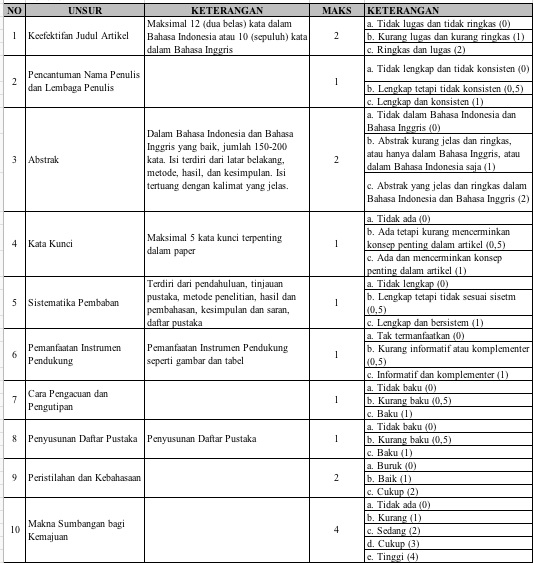
\includegraphics[width=1\textwidth]
      {figures/form1}}
      \caption{Form nilai bagian 1.}
      \label{form1}
      \end{figure}

	\begin{figure}[ht]
	      \centerline{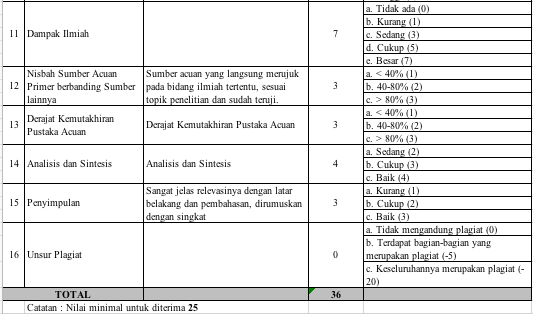
\includegraphics[width=1\textwidth]
	      {figures/form2}}
	      \caption{form nilai bagian 2.}
	      \label{form2}
	      \end{figure}


%next line adds the Bibliography to the contents page
\addcontentsline{toc}{chapter}{Bibliography}
%uncomment next line to change bibliography name to references
%\renewcommand{\bibname}{References}
\bibliography{references}        %use a bibtex bibliography file refs.bib
\bibliographystyle{plain}  %use the plain bibliography style

\end{document}

